%!TEX root = ../../Main.tex
\graphicspath{{Chapters/AssessmentTechniques/}}
%-------------------------------------------------------------------------------

\chapter{Assessment Techniques}

When collecting subjective image quality evaluations, numerous techniques exist. Three of the existing techniques (Absolute Category Rating, Degradation Category Rating, and Subjective Assessment Methodology for Video Quality) are described in this chapter. The benefits and drawbacks of using each assessment technique according to this project are also discussed in this chapter.

In a subjective image quality assessment scenario, an observer is presented for one or more stimulus (video or image) at a time and must rate the presented stimulus. 

\section{Absolute Category Rating} % (fold)
\label{sec:acr}

Absolute category rating (ACR) is a discrete rating system most commonly used for video quality testing \cite{ITU-TRecommendationP.9102008} but is also used for image quality testing \cite{Rouse2010}. The rating scale used in ACR has five categories; bad, poor, fair, good, and excellent. It can be a five-grade rating scale from 1 (bad) to 5 (excellent). This is referred to as the ACR-5. It can also consist of a higher number of grades like the ACR-9 or ACR-11 which are presented together with the ACR-5 in both \cite{ITU-TRecommendationP.9102008} and \cite{Rouse2010}. The labels are similar for all the ACR rating scales.

The process of ACR is to present each stimulus to the observer one at a time and only once. For stimuli being images, each image is presented to the observer for approximately 10 seconds followed by a gray screen from where the observer must rate the presented stimulus. The duration of the rating process depends on the rating scale but should not exceed 10 seconds. The process is illustrated in \autoref{fig:acr_method}.

\begin{figure}[H]
	\centering
	
\includegraphics[width = \columnwidth]{Img/ACR.pdf}
	\caption{The process of ACR. A stimulus is presented for 10 seconds followed by a gray screen from where the observer can rate the stimulus. This process is repeated until all stimuli have been rated.}
	\label{fig:acr_method}
\end{figure}

At the end of the process the observer should have assigned a rating score to all presented stimuli. When all observers have assigned a rating score for each stimulus a mean opinion score (MOS) is found for each stimulus by averaging all rating scores.

% section acr (end)

\section{Degradation Category Rating} % (fold)
\label{sec:dcr}

Degradation category rating (DCR) is similar to ACR a discrete rating system. This system is most commonly used when comparing an original stimulus with a modified version of the same stimulus \cite{ITU-TRecommendationP.9102008}. Due to the comparison, the labels for the DCR system is a little different; very annoying, annoying, slightly annoying, perceptible but not annoying, and imperceptible. Besides the labels, the rating scale is the same as in ACR where 1 is 'very annoying' and 5 is 'imperceptible'.

The process of DCR is much similar to the ACR system. The difference lies within the number of presented stimuli (one for ACR and two for DCR). First the observer is presented to the original stimuli followed by  the modified version. Both stimulus must be presented before the rating can take place. Between the two stimulus there is a short break of two seconds where the observer is presented to a gray screen. Similar to ACR the the presentation time for the stimulus is approximately 10 seconds when stimuli are images. As with ACR a MOS can be found for each stimulus. The process is illustrated in \autoref{fig:dcr_method}. 

\begin{figure}[H]
	\centering
	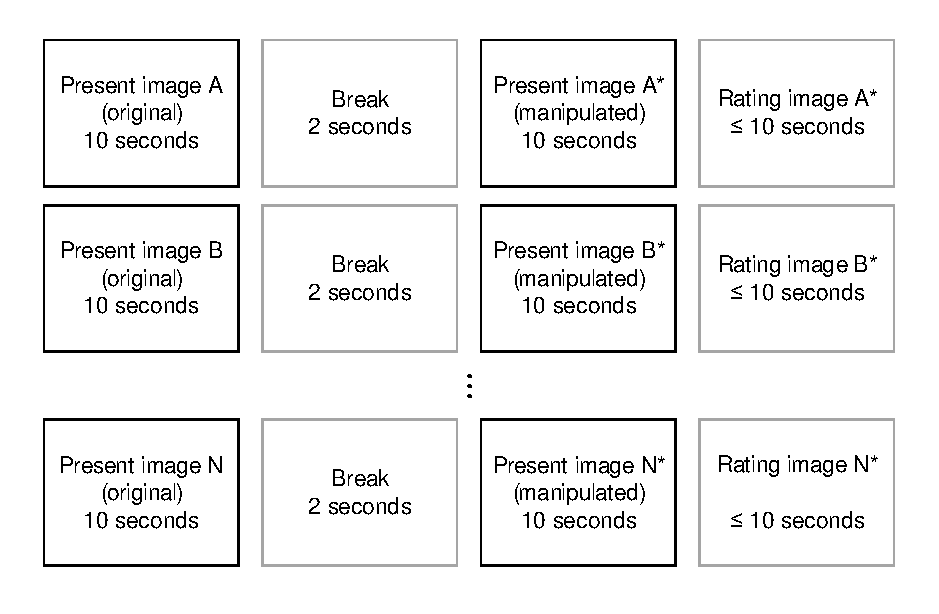
\includegraphics[width = 300pt]{Img/DCR.pdf}
	\caption{The process of DCR. Two stimuli are presented to the observer with a small break in between. The observer rates the second stimulus (modified) compared with the first stimulus (original).}
	\label{fig:dcr_method}
\end{figure}

% section dcr (end)

\section{Subjective Assessment Methodology for Video \\Quality} % (fold)
\label{sec:samviq}

Subjective assessment methodology for video quality (SAMVIQ) is another assessment technique which differs from the other assessment techniques in multiple ways even though the labels; bad, poor, fair, good, and excellent are the same as the ones used in ACR. As indicated by the name this technique is developed for use in video quality evaluation but has also been used for image quality evaluation as in \cite{Rouse2010}.

The rating scale in SAMVIQ differs from the two aforementioned techniques. The range of the scale goes from 0 to 100 where the label 'bad' is associated with the score 10 and the label 'excellent' is associated with the score 90. This scale has shown to be unnecessarily large and the observers ratings might be grouped in 5 or 9 groups over the rating scale range \cite{Rouse2010}.

The process of SAMVIQ also differs from earlier described techniques. In SAMVIQ the process is split into a number of scenes where each scene contains a number of different variations of the same stimulus. The explicit reference is the original stimulus and is known to the observer. The hidden reference is also the original stimulus but is unknown to the observer. Within a scene, the observer can browse freely between the different variations of the stimulus. Also the observer is able to evaluate the stimulus while observing it. When all stimulus has been rated, another scene might be presented and the process repeats itself. Notice that the order of the different variations of a stimulus changes for every scene. The process is illustrated in \autoref{fig:samviq_method}.

\begin{figure}[H]
	\centering
	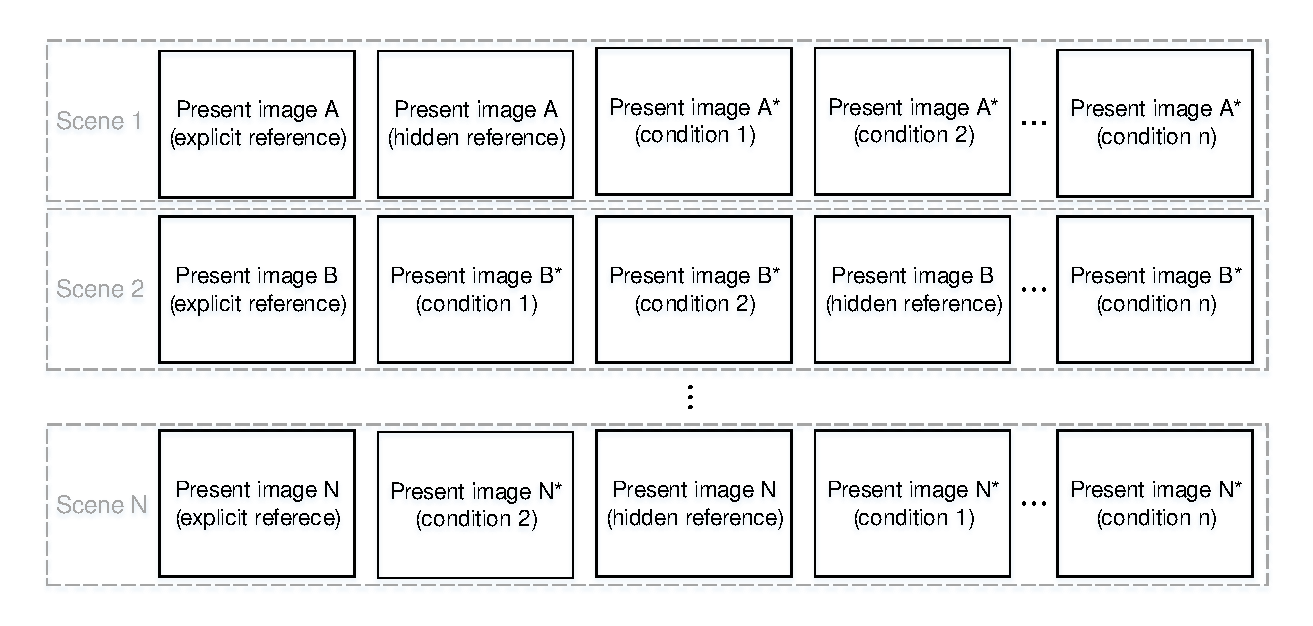
\includegraphics[width = \columnwidth]{Img/SAMVIQ.pdf}
	\caption{The process of SAMVIQ. Stimuli are split into scenes containing the same stimulus under different conditions (modified in different ways). All stimuli are rated before the observer gets to see the next scene.}
	\label{fig:samviq_method}
\end{figure}

The illustration in \autoref{fig:samviq_method} shows the use of a hidden reference. In SAMVIQ the use of a hidden reference is mandatory \cite{Kozamernik2005}.

% section samviq (end)

\section{Discussion} % (fold)
\label{sec:discussion}

The choice of assessment technique highly depends on the application which it is used for. In this project the focus is on evaluation of images which have been subject to a certain kind of lossy compression. The decrease in image quality, hence the error, between the compressed and uncompressed images, will vary according to the specific compression algorithm. The hardest thing to evaluate is the smaller errors which is difficult to see with the naked eye. A key aspect is therefore to provide the observer with the best opportunity to see and evaluate these types of errors.

The greatest benefit of ACR is that it is easy to understand and implement. The drawback, with respect to this project, is that the ACR does not have an explicit reference which is recommended in evaluations when the impairments of the images are small \cite{ITU-TRecommendationP.9102008}. Both DCR and SAMVIQ has the ability of using an explicit reference.

One difference of DCR and SAMVIQ is the rating scale. As mentioned before, experiments show that the rather large rating scale in SAMVIQ is superfluous \cite{Rouse2010} and the 5, 9 or 11 grade rating scale in DCR would be enough.

Despite the large rating scale the SAMVIQ assessment technique is chosen for this project due to the process of the technique. In DCR the reference is first shown followed by the image for evaluation and then these two steps are repeated. This is useful when evaluating many different images. In SAMVIQ the reference image together with different versions of this image are shown simultaneously. This is ideal for this project where the same image will be compressed in different ways.

A comparison of ACR and SAMVIQ showed that SAMVIQ needed less observers to obtain the same normalized confidence interval as ACR. The ACR-11 also needed fewer observers to obtain the same normalized confidence interval as the ACR-5 according to the same comparison \cite{Rouse2010}. This indicates that the 5 grade rating scale from ACR and DCR requires a higher number of observers than the 100 grade rating scale from SAMVIQ.

% section discussion (end)